\newpage
\section{Project Evaluation}
\subsection{Eclipse Plugin}
\subsubsection{UI Design choice}
Engineering the user interface of the Eclipse plugin involved numerous design choices, and several iterations of the plugin UI as it evolved with feedback.\\
The selection of big data framework configuration parameters to experiment and optimise is the most important part of the Big Data Auto-tuning tool. It is also the most complex part of the user interface due to the types of parameters available, which leads to different details, different forms of display and selection required. The different layouts considered were:
\begin{enumerate}
\item A table for available parameters, and a list of customised composite widgets, one for each parameter selected. Customised composite widgets have different fields and forms of displays to suit different types of parameters.
\item Two tables, one showing available parameters, and one showing selected parameters. Options and details for each selected parameter can be viewed and edited by double-clicking to bring up a pop up settings box.
\item Two tables, one showing available parameters, and one displaying selected parameters and corresponding options and details. The currently implemented UI as shown in Figure \ref{fig:param}.
\end{enumerate}
\begin{figure}[h]
\centering
\caption{Screen shot of parameter selection tab.}
\label{fig:param}
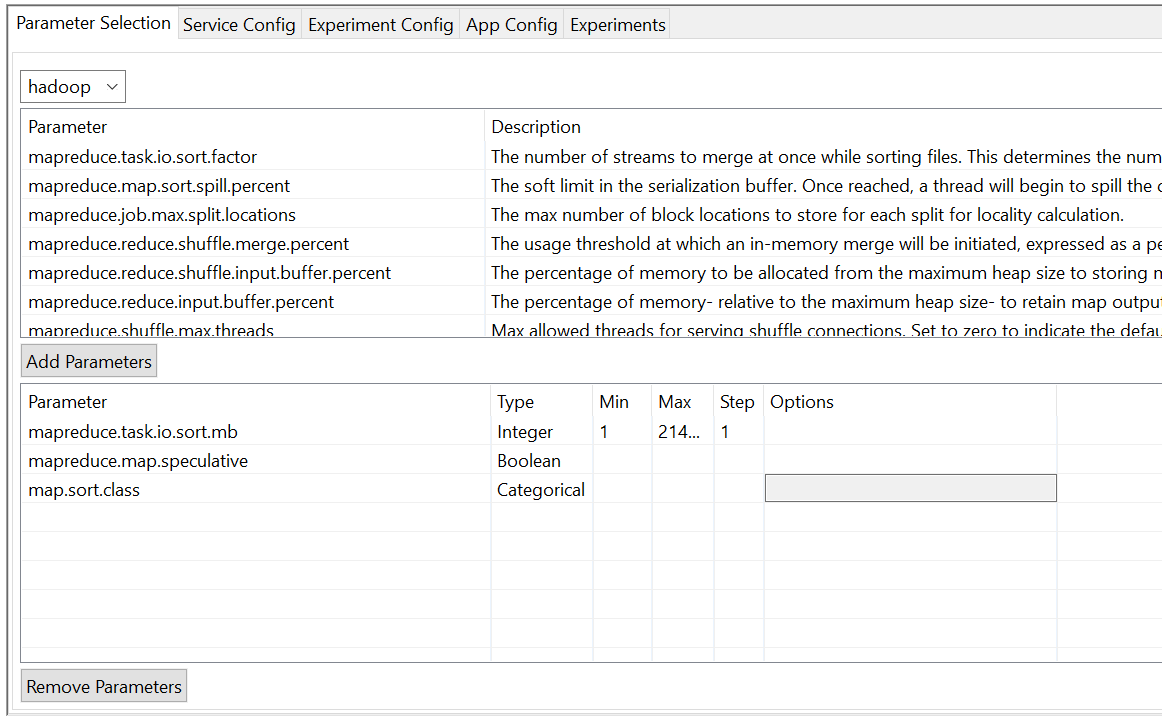
\includegraphics[width=\textwidth]{images/param.png}
\end{figure}
Each of the designs had their own merits and drawbacks:
\begin{enumerate}
\item Customised composite widgets are the most straight forward solution to handling parameters of different types. The ideal SWT widgets can be used to build up the composite for each parameter type. SWT has advanced built-in controllers to handle the layout and sizing of composites. However, the use of many individual widgets makes the layout crowded and bloated. Less parameters can be shown in the same space, and the different sizes and component for different parameters appears incoherent and messy to the user.
\item Having two tables gives the user interface a very coherent and clean layout. Tables are well suited to displaying strictly structured data. The incoherent details and options in the different types are hidden in the pop up setting boxes, that still allow each parameter type to be displayed using widgets that are an ideal fit. The drawbacks in this case is the inconvenience of having to double click and bring up a pop up box every time the user wishes to view or modify the details and options.
\item The current user interface layout is a balance between clean, coherency and convenience. The MultiCheckSelection Combo \cite{mcsc} was specifically designed to allow the options of categorical parameters to be semi-hidden with a drop-down menu, and fits the result into one cell. This allows the fitting of two tables that gives a clean, structured feel. There is a slight drawback in that forcefully attaching the created MultiCheckSelection Combo onto a table cell causes problems with the table's natural sizing, so some rows may not be automatically readjusted to their optimal size. It also is not entirely perfect in that the different types of parameters would leave blank columns used by other types of parameters. However, it was decided that these trade-offs are reasonable prices for a coherent layout that displays all information and details for each type of parameter concisely and conveniently. The table has added convenience of keyboard control and access using shortcuts such as the ``TAB'' and ``ENTER'' buttons to swiftly edit data.
\end{enumerate}
Considerable feedback was received for the plugin's user interface, which helped evolve the parameter selection tab over three iterations.\\
The first suggestion was a filter of available parameters by its corresponding big data framework. This idea was swiftly adopted because it is convenient to the user in that they only see relevant parameters. It also improves the performance of the plugin, by not creating unnecessary entries, hence reducing the number of objects created and managed. The filter function also help ensure correctness of the parameter selection, preventing mixing up of parameters of different big data frameworks in the selection.\\
The second suggestion centered on how the user ``selects'' a parameter to be experimented upon. The original implementation uses a drag and drop gesture, where parameters can be dragged into the selected table, or dragged back to the available table. However, the performance of this gesture based system was problematic. It is believed that the custom combo used in one of the tables causes problems that may be due to the dynamic resizing that occurs whenever the table is changed. The feedback also suggests that a switch to having ``Add Parameter'' and ``Remove parameter'' buttons would be convenient for a broader group of developers especially those who are using laptops without a proper mouse, or those who prefer to access UI components using the keyboard shortcuts. The drag and drop gesture does not work well for these user groups.\\
However, the additional buttons do create a problem, that they do need to be pressed when the users wishes to change selection. Previously, the user only had to perform one dragging jesture. To compensate, a double-click listener is added to the final version of the Eclipse plugin, so that the user has a more convenient way of selection.

\newpage
\subsubsection{UI Implementation Choices}
Choice of framework and tools to work with is the most crucial when implementing the user interface. As the Big Data Auto-tuning tool is to be integrated with the Eclipse based DICE IDE environment, any work must be based on SWT. The approaches can be pure SWT or JFace on top of SWT:
\begin{itemize}
\item Eclipse SWT Standard Widget Toolkit \cite{swt}
	\begin{itemize}
	\item Provides a common API across wide platform
    \item Uses native widgets from the platform
    \item Maintains native look and feel of user interface
    \item Faster, more responsive and lighter system resource usage
    \item Available as standard with Eclipse plugin development environment
    \item Designed for Windows platform, other ports may be less efficient
    \item Exposed to platform-specific bugs in the native library
    \item Requires programmer to work with lower level native GUI library
    \item Does not provide MVC architecture
	\end{itemize}
\item JFace \cite{jface}
	\begin{itemize}
    \item brings Model-View-Controller architecture to SWT
	\item provides adaptors to handle the common code for handling widget events
	\item provides Actions to allow users to define their own behavior and to assign that behavior to specific components, e.g. menu items, tool items, push buttons, etc.
	\item Provides registries that hold Images and Fonts
	\item Defines standard dialogs and wizards, and defines a framework for building complex interactions with the user
	\end{itemize}
\end{itemize}
The current implementation forgoes the majority of JFace uses, because the Eclipse plugin of the Big Data Auto-tuning tool functions mainly to obtain user input, and does not have to do too much processing on the input. The logic and data required in the plugin is not of the complexity to merit the use of the full MVC architecture, which although an elegant solution, would take additional time and effort to set up. The current implementation has a general architecture the separate the concerns of front end components responsible for displaying the user interface, and backend components to handle the integration functionalities. It is not envisioned that there will be significant extensions to the functionality of the Eclipse plugin that requires complex logic in the future. The Eclipse plugin also does not require any images or fonts, dialogs or wizards. Hence for the sake of simplicity, the only JFace components used in the current implementation are the adaptors to handle widget events.\\

Another architecture choice is on the use of the SWT's events and listener architecture. Under the listener architecture, each SWT component should be \textit{listening} to the events that relate to them. This is done by adding itself to the trigger's listener list. When an event occurs, it is broadcasted to all listeners in the list, by calling the corresponding method on the listener. It is up to each of the listener components to decide how it should react to the event by overriding the method.\\
The alternative implementation is for a central controller to react to events, and then execute actions on the components. Instead of the listeners subscribing to event broadcasts, the linking is reversed with the central controller holding information about all the relevant component it controls.\\
As detailed in Figure \ref{fig:paramtab} in the implementation section, the current implementation is a combination of both approaches. There is not one central controller that coordinates all actions, but instead each key button on the tab controls its relevant actions. Buttons in the tab have listeners to detect when they are pressed, and then they control other components to execute the desired action. These other components include the tables, items in the tables and the customised selection combos attached to the tables. These components are stored in maps that are globally accessible throughout plugin context, so that controllers can access the relevant objects and data.\\
For example, to manage the removal of selected parameters:
\begin{enumerate}
\item The ``Remove parameter'' button listens for the event that it has been pressed
\item The listener method then queries the selected parameters table for a list of highlighted entries to be removed
\item Look up the maps to find the linked parameter and any linked graphical components such as customised selection combos. 
\item Calls the disposal method on the linked components and the entry itself, and creates a new entry for the parameter in the available parameters table
\end{enumerate}
This implementation is easy to understand as a programmer, and easy to debug and make modifications because all of the actions relating to this event of ``removing a parameter'' is centralised at that button.\\
An alternative implementation using the listener architecture:
\begin{enumerate}
\item Each entry in the selected parameters table subscribe to listen to the ``Remove parameter'' button
\item Each related graphical component to the entry listen to the entry
\item When the button is pressed all entries in the table are notified
\item Each entry then checks if it is highlighted to be removed
\item If the entry is highlighted, it in turn notifies its related graphical components
\item The graphical components will react by removing themselves
\end{enumerate}
This implementation does not require extra memory space for global maps, but will create lists of listeners for each component. It also does not require looking up the map to find corresponding components, but sends the notification to all components instead, leaving it to the component to decide if it needs to react. Due to the distributed nature of this approach, it is harder to debug what has gone wrong in the reaction to ``removing a parameter''. Developers have to update many components to make a single modification to the behaviour.\\
For these reasons, the choice was made to not fully implement the listener architecture down to the lower levels.

\newpage
\subsubsection{Contribution to SWT}
The Eclipse Foundation's SWT Standard Widget Toolkit is open sourced and maintained by the community. In following of the open source spirit, the MultiSelectionCombo developed as part of this project has been released.\\
The MultiSelectionCombo was developed to allow selecting multiple values from a list of categorical options, required by to display and specify categorical parameters in the Big Data Auto-tuning tool. However it can be applied to any general use case where its features are required:
\begin{itemize}
\item shows an arbitrarily long list of options on a temporary drop down list
\item each item on the list can be selected by selecting the corresponding check box button
\item minimise to fixed size text display of selected options
\end{itemize}
\begin{figure}[h]
\centering
\caption{Screen shot of MultiSelectionCombo.}
\label{fig:screenshot}
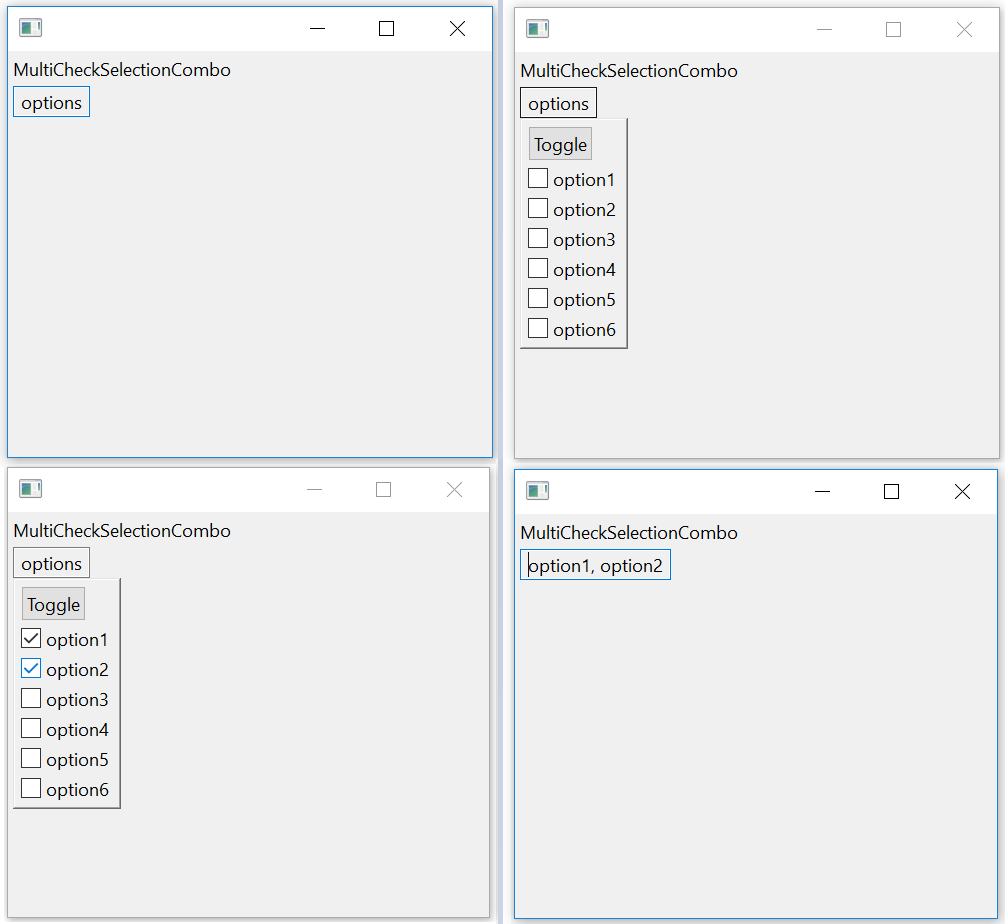
\includegraphics[width=\textwidth]{images/screenshot.png}
\end{figure}
The MultiSelectionCombo is similar to the SWT Combo, but it was built from scratch because SWT conventions dictate that the Combo class cannot be extended. The Combo class does not allow multiple values to be selected, and does not contain the check box buttons required, hence there is a need for the creation of a new widget.\\
The case for this widget is further strengthened by the strong and persistent request for a combo that fits this specification - since as early as 2007 \cite{2007}, there has been an activity in the community seeking for such a widget, and the requests have not stopped in the following years, up to 2015 \cite{2015}.\\
There have been attempts and small, specific implementations of such a widget, but none with the clear objective of developing a general, re-usable SWT-standard widget \cite{prev}. The previous attemps also do not follow SWT conventions of standardised API, and fail to address efficiency, memory space and de-allocation considerations. The MultiCheckSelectionCombo is created with support of all the API provided by the comparable original SWT Combo class. The MultiCheckSelectionCombo has clear documentation, simple and efficient data structure, and robust implementation of memory de-allocation to maintain performance. The detailed Javadoc of the MultiCheckSelectionCombo is available in the \href{https://lawhcd.github.io/SWTMultiCheckSelectionCombo/}{link} \cite{javadoc}, with the released source code available on \href{https://github.com/lawhcd/SWTMultiCheckSelectionCombo}{GitHub} \cite{mcsc}.

\newpage
\subsubsection{Eclipse Plugin Backend}
Big data framework configuration parameters are prone to change. Therefore it was an obvious decision to leave the specifics of configuration parameters out of the source code of the Big Data Auto-tuning Tool. The parameters are read from the \textit{params.xml} file instead.\\
Currently one file contains all available parameters across all big data frameworks. It can be sensible to split into a different parameter file for each big data framework. That approach can lead to slightly faster loading time when showing parameters of selected big data framework, because the data is already filtered and does not require processing. However, for simplicity and convenience of implementation, it had been decided that the small performance gain was insignificant, given a list of parameters in the order of tens in total. Should the tool be extended to support more big data frameworks, or more configuration parameters become available, the option to split into multiple files should be re-considered.\\
It is also worth discussing the selection of parameters available in the Big Data Auto-tuning tool. The criteria for the inclusion of a configuration parameter was that it was ``performance related''. There has not been sufficient background research to clearly prove which parameters had significant impact on performance, and the selection was purely based on details provided by the official documentation. Given more time, the ``performance relatedness'' of a parameter could have been evaluated to take a more formulaic and scientific approach to selecting parameters to make available in the tool. An alternative would be to include all parameters and make it the developer's responsibility to select sensible options. However, that would be a backwards step from the aim to create and integrated development environment that aids developers with little or no knowledge to explore and improve the performance of big data applications.

\newpage
\subsection{Integration: Eclipse, Jenkins, BO4CO, Testbed}
\subsubsection{Eclipse and Jenkins Integration}
Existing state of the art integration between Eclipse and Jenkins is provided by the Hudson/Jenkins Mylyn Builds Connector \cite{mylyn}. It does not support triggering of parameterised Jenkins builds from Eclipse, and hence also does not support the inclusion of file parameters in the trigger request.\\
In the wider scope, Jenkins remote API supports remote triggering of parameterised builds with file parameters \cite{pbuild}, but there lack of documentation makes the task challenging.\\
The Big Data Auto-tuning tool is the first fully integrated tool that enables remote triggering of a Jenkins parameterised build with a file parameter from the Eclipse IDE. Although it is specifically designed to trigger the Configuration Optimisation process in its current form, it can be extended to support general use cases.

\subsubsection{Bug Fixes and Improvements to BO4CO}
A number of bugs were found in BO4CO code and fixed. Due to the complexity and tightly coupled nature of the system, with dependencies that extend beyond the code base into the services that are used to deploy experiments,  parts of the debugging was time consuming. As the development was done in MATLAB, there were no advanced debugging and testing tools such as Java's JMock tester, which would have helped to eliminate problems and the very long running time of actually deploying real experiments on the Storm cluster to test. (At least 20 minutes per test).\\
Most of the fixes applied are ideal solutions which retain the intended functionality, are efficient and well designed. However, the fix to the erroneous hard-coded reading of service configurations in the initialisation step (\textit{init.m}) should be regarded as a temporary fix, as a truly general solution has not been implemented due to time constraints.\\
There is a limitation on the validity of these fixes, as the testing has only been conducted on the source code run with a Storm cluster. There have been no tests run with a compiled version of the tool, and no tests with a Hadoop cluster, due to the lack of these resources. A compiled version was unavailable due to MATLAB licensing issue.

\newpage
\subsubsection{Extension on BO4CO}
BO4CO Configuration optimisation tool is a ground breaking approach to help developers of big data applications automatically improve the performance by experimenting on configuration parameters. It was limited to experimenting with numerical parameters. This work to extend its functionality to categorical and boolean parameters is yet another ground breaking step, such that it can now be said that the BO4CO Configuration optimisation tool can work with all existing big data framework parameters. The investigation concluded that all parameters for all big data frameworks considered in the DICE project are of one of the four supported types: Integer, Percentage, Categorical or Boolean. Hence this removes a significant restriction on the vision of a fully integrated tool that automates the entire process of configuration optimisation.\\
It is believed that the algorithm has no problems dealing with categorical and boolean data types, despite the fundamental differences with numerical data types. The algorithm processes index values of the options provided, instead of dealing directly with the value of the option itself \cite{bo4co}. Despite the fact the options for numerical parameters may show a sense of pattern (e.g. an increasing order), while categorical and boolean parameters are perceived to have no such ordering, the algorithm does not rely on such ordering to function, so should function correctly for these new data types. It is accepted that the ordering of numerical options does helped the performance of the tool, but in the long run the results of non-ordered options are believed to converge as well.\\
Due to time constraints, it was not possible to draw any meaningful statistical measure of how well the tool performs with Categorical and Boolean parameters. However, the implementation has been validated - the tool is able to process and deploy experiments with Categorical and Boolean parameters, with no adverse effect to the existing functionality that supported numerical parameters.

\subsubsection{Jenkins and BO4CO MATLAB Integration}
Jenkins provides the ability to automatically execute the tool in a remote server, monitor the progress and retrieve the results any time after the experiments have completed. The remote, automatic and self-contained nature of a Jenkins server is crucial to the Big Data Auto-tuning Tool, as the configuration optimisation experiments can run for any time from tens of minutes up to tens of hours. It would be a significant inconvenience if the developer had to run the process on the local machine, and possibly keep the Eclipse plugin open for the whole duration.\\
The work on this integration was specific for the use case, but it provides a consolidated approach that can be generalised to all developers who wish to set up Jenkins automation and continuous integration for running and testing MATLAB source code in a Windows environment. There has not been a comprehensive and detailed solution for this setting, with the community documentation \cite{matlabjenkins} only introducing the approach for Linux environments, that does not directly work in a Windows set up.\\